\chapterimage{habowangxingkong_127202_10}% Chapter heading image

\chapter{Week6}

\section{Tuesday}\index{week6_Tuesday_lecture}
\subsection{Summary of last two weeks}
In the first two weeks, we have learnt how to solve linear system of equations $\bm{Ax}=\bm b$. To understand this equation better, we learn the definition for matrices and vector space. Matrices calculation involve vectors, the columns $\bm{Ax}$ are linear combination of $n$ vectors--columns of $\bm{A}$. \\
\subsubsection{Determinants}
And then we learn how to describle the \emph{quantity of a matrix}--determinant. The determinant of a square matrix is a single number. That number contains an amazing amount of information about the matrix. There are three main points about determinant:
\begin{itemize}
\item
\textit{Determinants is related to invertibility, rank, eigenvalue, PSD$,\dots$}
\item
$\det(\bm{AB})=\det(\bm A)\det(\bm B).$
\item
\textit{The square matrix $\bm A$ is invertible} if and only if $\det(\bm A)\ne 0.$
\end{itemize}

\subsubsection{Linear Transformation}
Linear transfromation is another important topic. The matrix multiplication $T(\bm v)=\bm{Av}$ gives a lienar transformation. If we consider a vector as a point in a vector space, then \textit{the linear transformation allows movements in the space}. It ``transforms'' vector $\bm v$ to another vector $\bm{Av}$. In view of linear transformation, we can understand $\det(\bm{AB})=\det(\bm A)\det(\bm B)$ better:
\[
\det(\bm A)=\text{Volumn of $\bm{Ak}$, where $\bm k$ is a unit cube.}
\]
If we transform the $\bm k$ by $\bm A$ secondly by $\bm B$, actually, it has the same effect of transforming $\bm k$ by $\bm{BA}$.
\begin{figure}[H]
\centering
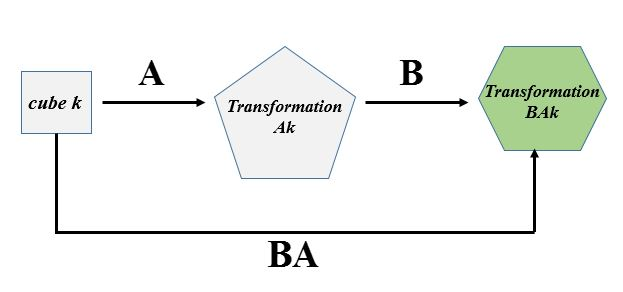
\includegraphics[width=10cm]{week6/determinant}
\caption{Transformation of a vector by $\bm A$, then by $\bm B$ has the same effect by $\bm{BA}$.}
\end{figure}
Hence if we denote the volumn on a graph, we find the volumn of $\bm B(\bm{Ak})$ is exactly the same as $(\bm{BA})\bm k$. Hence we have $\det(\bm B)\det(\bm A)=\det(\bm{BA})$.\\
Morevoer, $\det(\bm A)=0\Longleftrightarrow
\text{Volumn of $\bm{Ak}=0$}\Longleftrightarrow
\dim(\bm{Ak})=0.$\\
Cramer's Rule also has geometric meaning, which will not be talked in this lecture. (In big data age, people will not use cramer's rule frequently.)\\
Linear transformation has a matrix representation under certain basis. How to transform one basis into another basis? We have to use \textit{similar matrices as matrix representation}.
\subsubsection{Orthogonality}
Why we learn orthogonality? It has two motivations:
\begin{enumerate}
\item
Linear independence between vectors
$\Longleftrightarrow\text{Angle}\ne0\degree.$\\
Then we are interested in the special case:
orthogonal$\Longleftrightarrow\text{Angle}=90\degree$.
\item
Solving least squares (linear regression).\\
Input: $x =$age of propellant, Output: $y = $shear strength.\\
Our data contains $S=\{(x_1,y_1),\dots,(x_{n},y_{n})\}$, $n=20$ samples.\\
We want to find a best line that fit the data:
\begin{figure}[H]
\centering
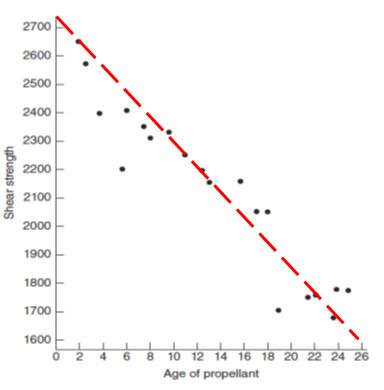
\includegraphics[width=5cm]{week6/regression}
\caption{The relationship between $x$ and $y$.}
\end{figure}
In other words, we want to find $\bm x$ s.t.
\[
    (\tikzmark{identity}{$\bm A$}\tikzmark[red]{G}{$\bm x$}
    \approx\tikzmark[purple]{C}{$\bm b$})
\]
\begin{tikzpicture}[overlay, remember picture,node distance =1.5cm]
    \node (identitydescr) [below left=of identity ]{age};
    \draw[,->,thick] (identitydescr) to [in=-90,out=90] (identity);
    \node[red] (Gdescr) [below =of G]{coefficient};
    \draw[red,->,thick] (Gdescr) to [in=-90,out=90] (G);
    
    \node[purple] (Cdescr) [below right =of C]{strength};
    \draw[purple,->,thick] (Cdescr) to [in=-90,out=90] (C.south);
\end{tikzpicture}
\end{enumerate}
\newpage
The general least square problem is given by:
\[
\min_{\bm x\in\mathbb{R}^{n}}\|\bm{Ax}-\bm b\|^2
\]
where $\bm b\in\mathbb{R}^{m}$.
\begin{itemize}
\item
If $m=n$, this optimization problem is converted into find the solution to equation $\bm{Ax}=\bm b$.
\item
Otherwise, the least square solution must satisfy $\frac{\partial }{\partial \bm x}\|\bm{Ax}-\bm b\|^2=\bm 0$.
\[
\implies\bm A\trans\bm A\bm x=\bm A\trans\bm b.\qquad\text{(\emph{normal equation.})}
\]
\end{itemize}
This potimization problem also has geometric meaning:
\begin{figure}[H]
\centering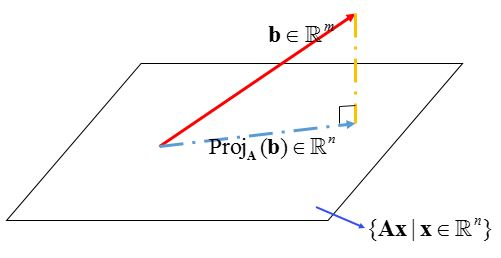
\includegraphics{week6/least_square}
\caption{Least square problem: find $\bm x$ such that $\bm{Ax}=\Proj_{\bm A}(\bm b).$}
\end{figure}
So you need to memorize we only need to find $\bm x$ such that $\bm{Ax}=\Proj_{\bm A}(\bm b)$.\\
But how to find $\Proj_{\bm A}(\bm b)$? You can write it as inner product:
\[
\Proj_{\bm A}(\bm b)=\bm A\frac{1}{\inp{\bm A}{\bm A}}\inp{\bm A}{\bm b}
=\bm A(\bm A\trans\bm A)^{-1}\bm A\trans\bm b.
\]
\begin{remark}
\begin{itemize}
\item
The projection of $\bm b$ onto a vector $\bm a$ is given by:
\[
\Proj_{\bm a}(\bm b)=\frac{\inp{\bm a}{\bm b}}{\inp{\bm a}{\bm a}}\bm a
\]
Since the factor $\frac{\inp{\bm a}{\bm b}}{\inp{\bm a}{\bm a}}$ is a scalar, you can also write the projection as:
\[
\Proj_{\bm a}(\bm b)=\bm a\frac{\inp{\bm a}{\bm b}}{\inp{\bm a}{\bm a}}
\]
\item
However, the projection of $\bm b$ onto a subspace $\{\bm{Ax}|\bm x\in\mathbb{R}^{n}\}$ is given by
\[
\Proj_{\bm A}(\bm b)=\bm A\frac{1}{\inp{\bm A}{\bm A}}\inp{\bm A}{\bm b}
\]
We \emph{cannot} write this projection as $\frac{1}{\inp{\bm A}{\bm A}}\inp{\bm A}{\bm b}\bm A$, since the factor $\frac{1}{\inp{\bm A}{\bm A}}\inp{\bm A}{\bm b}$ is a vector instead of a scalar.
\enlargethispage{1cm}
\end{itemize}
\end{remark}
The least square solution is given by
\[
\bm x=(\bm A\trans\bm A)^{-1}\bm A\trans\bm b.
\]
If $\bm A=\bm Q$, where $\bm Q$ is a \textit{orthogonal matrix}, then the solution is converted as 
\[
\bm x=\bm Q\trans\bm b.
\]
\subsection{Eigenvalues and eigenvectors}
\subsubsection{Why do we study eigenvalues and eigenvectors?}
\begin{itemize}
\item
\emph{Motivation 1: }If we consider matrices as the \textit{movements} (linear transformation) for \textit{vectors} in vector space. Then roughly speaking, \textit{eigenvalues} are the \textit{speed} of the movements, \textit{eigenvectors} are the \textit{direction} of the movements
\item
\emph{Motivation 2: }We know that linear transformation has different matrix representation for different basis. But which representation is \emph{simplest} for one linear transformation? This section gives us answer to this question.
\end{itemize}
When vectors are multiplied by A, almost all vectors change direction. If $\bm x$ has the same direction as $\bm{Ax}$, they are called \emph{eigenvectors}.
\[
\text{\emph{The key equation is }}\bm{Ax}=\lambda\bm x,\qquad\text{\emph{The numebr $\lambda$ is the eigenvalue of $\bm A$.}}
\]
\begin{definition}[Eigenvectors and Eigenvalues]
Let $\bm A$ be $n\times n$ matrix. A scalar $\lambda$ is an \emph{eigenvalue} of $\bm A$ iff $\exists$ a vector $\bm x\ne \bm 0$ s.t. $\bm{Ax}=\lambda \bm x$. The vector $\bm x$ is called an \emph{eigenvector} (corresponding to $\lambda$.)
\end{definition}
\begin{example}\qquad\\
\begin{gather*}
\bm A=\begin{bmatrix}
4&-2\\1&1
\end{bmatrix}\qquad\bm x=\begin{bmatrix}
2\\1
\end{bmatrix}\\
\bm{Ax}=\begin{bmatrix}
6\\3
\end{bmatrix}=3\begin{bmatrix}
2\\1
\end{bmatrix}=3\bm x.
\end{gather*}
$\lambda=3$ is the eigenvalue of $\bm A$.\\
$\bm x=\begin{bmatrix}
2\\1
\end{bmatrix}$ is the eigenvalue of $\bm A$ associated with $\lambda=3.$
\end{example}
\begin{proposition}
If $\bm x$ is an eigenvector of $\bm A$, so is $\alpha\bm x$ for all \textit{nonzero} scalar $\alpha$. (These vectors have the same eigenvalue.)
\end{proposition}
\subsubsection{Calculation}
How to find $\lambda$ and $\bm x$? In other words, how to solve the nonlinear equation $\bm{Ax}=\lambda\bm x$, where $\lambda$ and $\bm x$ are unknowns? If we can know the eigenvalues $\lambda$, then we can solve the system $(\lambda\bm I-\bm A)\bm x=\bm 0$ to get the corresponding eigenvectors.\\
But how to find eigenvalues? $\bm{Ax}=\lambda\bm x$ has a nonzero solution $\Longleftrightarrow$$(\lambda\bm I-\bm A)\bm x=\bm 0$ has a nonzero solution $\Longleftrightarrow$ $(\lambda\bm I-\bm A)$ is singular $\Longleftrightarrow$$\det(\lambda\bm I-\bm A)=0.$\\ This is how to recognize an eigenvalue $\lambda$:
\begin{proposition}
The number $\lambda$ is the eigenvalue of $\bm A$ if and only if $\lambda\bm I-\bm A$ is singular.
\begin{equation}
\text{\emph{Equation for the eigenvalues}}
\qquad
\det(\lambda\bm I-\bm A)=0.
\end{equation}
\end{proposition}
\enlargethispage{1cm}
\begin{definition}[characteristic polynomial]
Define $P_{\bm A}(\lambda):=\det(\lambda\bm I-\bm A)$. \\Then $P_{\bm A}(\lambda)=\det(\lambda\bm I-\bm A)$ is called the \emph{characteristic polynomial} for the matrix $\bm A$.\\ And the equation $\det(\lambda\bm I-\bm A)=0$ is called the \emph{characteristic equation} for the matrix $\bm A$.\\ If $P_{\bm A}(\lambda^{*})=0$, then we say $\lambda^*$ is the root of $P_{\bm A}(\lambda)$.
\end{definition}
The roots of $P_{\bm A}(\lambda)$ are the \emph{eigenvalues} of $\bm A$. $\forall\bm x\in N(\lambda\bm I-\bm A)$ (\textit{eigenspace}) is an eigenvector associated with $\lambda$.
\newpage
\begin{example}
Find the eigenvalues and eigenvectors of $\bm A=\begin{bmatrix}
3&2\\3&-2
\end{bmatrix}$.\\
\begin{gather*}
\det(\lambda\bm I-\bm A)=\begin{bmatrix}
\lambda -3&-2\\-3&\lambda+2
\end{bmatrix}=0.\\
\implies (\lambda+3)(\lambda-2)-6=0.
\implies \lambda^2-\lambda-12=0.\implies
\lambda_1=4\quad\lambda_2=-3.
\end{gather*}
Eigenvalues of $\bm A$ are $\lambda_1=4\text{ and }\lambda_2=-3.$\\
In order to get eigenvectors, we solve $(\bm A-\lambda\bm I)\bm x=\bm 0$:
\begin{itemize}
\item
For $\lambda_1$, $(\bm A-\lambda_1\bm I)\bm x=\begin{bmatrix}
-1&2\\3&-6
\end{bmatrix}=\bm 0$.
\[
\implies \bm x=\begin{bmatrix}
2x_2\\x_2
\end{bmatrix}=x_2\begin{bmatrix}
2\\1
\end{bmatrix}
\]
Hence any $\alpha\begin{bmatrix}
2&1
\end{bmatrix}\trans$ $(\alpha\ne0)$ is the eigenvector of $\bm A$ associated with $\lambda_1=4.$
\item
For $\lambda_2$, similarly, we derive
\[
\bm x=\begin{bmatrix}
-x_2\\3x_2
\end{bmatrix}=x_2\begin{bmatrix}
-1\\3
\end{bmatrix}
\]
Hence any $\beta\begin{bmatrix}
-1&3
\end{bmatrix}\trans$ $(\beta\ne0)$ is the eigenvector of $\bm A$ associated with $\lambda_2=-3.$
\end{itemize}
\end{example}
\subsubsection{Possible difficulty: how to solve $\det(\lambda\bm I-\bm A)=0$?}
$P_{\bm A}(\lambda)$ is a characteristic polynomial with degree $n$. Actually, we can write $P_{\bm A}(\lambda)$ as:
\[
P_{\bm A}(\lambda)=\lambda^n-a_1\lambda^{n-1}+a_2\lambda^{n-2}-\dots+(-1)^{n}a_n
\]
When $n$ increases, it's hard to find its roots:
\begin{itemize}
\item
When $n=2$, solution to $ax^2+bx+c=0$ has \textit{closed form}, which means we can express $x$ in terms of $a,b,c$ directly.
\item
When $n=3$, solution to $ax^3+bx^2+cx+d=0$ has \textit{closed form}, which has been proved in $15$th century.
\item
When $n=4$, solution to $ax^4+bx^3+cx^2+dx+e=0$ also has \textit{closed form}.
\item
However, when $n\ge5$, the characteristic equation has \textit{no closed form} solution, which has been proved by Galois and Abel.
\end{itemize}
Although we cannot find closed form solution for large $n$, does there exist such solution which is not closed form? Gauss gives us the answer:
\begin{theorem}[Fundamental theorem of algebra]
Every nonzero, single variable, degree $n$ polynomial with \textit{complex coefficients} has \textit{exactly} $n$ complex roots. (Counted with multiplicity.)
\end{theorem}
What's the meaning of \textit{multiplicity?}\\ For example, the polynomial $(x-1)^2$ has one root 1 with multiplicity 2.\\
\newpage
\emph{Implication: }\\
Hence every polynomial $f(x)$ could be written as
\begin{align*}
f(x)&=a_nx^n+a_{n-1}x^{n-1}+\dots+a_1x_1+a_0\\
&=a_n(x-x_1)(x-x_2)\dots(x-x_n)
\end{align*}
where $x_i$'s are roots for $f(x)$.\\
Moreover, \emph{$P_{\lambda}(\bm A)$ has exactly $n$ roots, or say, $\bm A$ has $n$ eigenvalues.(counted with multiplicity.)}
\begin{remark}
Exact roots are almost impossible to find. But approximate roots (eigenvalues) can be find easily by numerical algorithm. (such as Newton's method.)
\end{remark}
\subsection{Products and Sums of Eigenvalue}
Suppose $P_{\bm A}(\lambda)=\det(\lambda\bm I-\bm A)$ has $n$ roots $\lambda_1,\dots,\lambda_n$, then we obtain:
\begin{equation}
P_{\bm A}(\lambda)=\det(\lambda\bm I-\bm A)=(\lambda-\lambda_1)\dots(\lambda-\lambda_n)
\label{characteristic}
\end{equation}
Why the coefficient for $\lambda^{n}$ is 1 in equation (\ref{characteristic})? If we expand $\det(\lambda\bm I-\bm A)$, we find
\begin{equation}
\det(\lambda\bm I-\bm A)=\begin{vmatrix}
\lambda-a_{11}&-a_{12}&\dots&-a_{nn}\\
-a_{21}&\lambda-a_{22}&\dots&-a_{2n}\\
\vdots&\vdots&\ddots&\vdots\\
-a_{n1}&\dots&\dots&\lambda-a_{nn}
\end{vmatrix}
\label{characteristic_det}
\end{equation}
So $\lambda$ only appears in diagonal. If we expand the determinant, the coefficient is obviously 1.\\
Moreover, in $(\ref{characteristic})$, the coefficient of $\lambda^{n-1}$ is
\[
-(\lambda_1+\lambda_2+\dots+\lambda_n)
\]
In $(\ref{characteristic_det})$, $\lambda^{n-1}$ only appears among $(\lambda-a_{11})(\lambda-a_{22})\dots(\lambda-a_{nn})$. Hence the coefficient of $\lambda^{n-1}$ is
\[
-(a_{11}+a_{22}+\dots+a_{nn})
\]
Consequently, we derive
\[
\sum\lambda_i=\text{\emph{trace}}=\sum a_{ii}
\]
The sum of the entries on the main diagonal is called the \emph{trace} of $\bm A$.\\
If we let $\lambda=0$ in $(\ref{characteristic})$, then we obtain $\det(-\bm A)=(-1)^n\lambda_1\lambda_2\dots\lambda_n$.  \\
And obviously, $\det(-\bm A)=(-1)^{n}\det(\bm A)$.\\
Hence $(-1)^{n}\det(\bm A)=(-1)^n\lambda_1\lambda_2\dots\lambda_n\implies
\det(\bm A)=\lambda_1\lambda_2\dots\lambda_n.$
So we have two useful conclusions:
\begin{theorem}
\emph{\textit{The product of the $n$ eigenvalues equals the determinant.}}\\
\emph{\textit{The sum of the $n$ eigenvalues equals the sum of the $n$ diagonal entries.}}
\end{theorem}
\subsection{Application: Page Rank and Web Search}
If we do keyword search on google, every keyword will return 20k pages. But how to generate more useful pages for us? Our goal is to \textit{compute a vector $\bm x=\begin{bmatrix}
x_1&x_2&\dots&x_n
\end{bmatrix}$ in $\mathbb{R}^{n}$, each $x_i$ represents the importance of the page.} Then we only need to generate the most important pages for us.\\
\newpage
The information we use: links.\\
We use the number of links to judge whether a page is important. For example,
\begin{itemize}
\item
A page \textit{linked to by $10^5$ pages} is more important than a page \textit{linked by $10$ pages}.
\item
If two pages \textit{both linked to by $100$ pages}, are they the same important?\\
The answer is no. For example, in your own blogs, if you create $100$ pages that all link to your home page, then obviously your home page is not so important. These $100$ pages are created by yourself, which are called \emph{fake pages}.
\end{itemize}
We do the following assumptions:
\begin{itemize}
\item
Assume we have $100n$ people are visiting pages. We have $n$ pages.
\item
We assume every page have $100$ visitors. They follow the links on that page.
\item
And we assume \textit{multiple of links are equally split.} (For example, if one page have $5$ links, then there will be $100/5=20$ people follow each link.)
\end{itemize}
To start with, the distribution of people for $n$ pages is given by:
\[
\bm x^0=\begin{pmatrix}
x_1^0\\x_2^0\\\vdots\\x_n^0
\end{pmatrix}
\]
We assume the probability people will go from page $j$ to page $i$ is $a_{ij}$.\\
Question: If page $j$ links to by $5$ pages, what's $a_{ij}$?\\
Answer: due to assumption 3, roughly speaking, $a_{ij}=\frac{1}{5}$.\\
However, this answer is not absolutely right. Since assumption is not always true. If we consider \textit{stochastic process}, then $a_{ij}$ is given by:
\[
a_{ij}=0.85\times\frac{1}{5}+0.15\times\frac{1}{n}.
\]
If we write matrix $\bm A=\begin{bmatrix}
a_{ij}
\end{bmatrix}_{1\le i,j\le n}$, then the $(i,j)$ entry of $\bm A$ represents the probability that a random Web surfer will link from page $j$ to page $i$.
\\
Next step distribution:\\
Hence when each surfer follow one link of the pages, the distribution of people among pages is given by
\[
\bm x^1=\bm A\bm x^0=\begin{pmatrix}
x_1^1\\x_2^1\\\vdots\\x_n^1
\end{pmatrix}
\]
In general, we obtain $\bm x^{k+1}=\bm A\bm x^{k}$.\\
If the sequence $\{\bm x^k\}$ converges, then take the limit $k\rightarrow\infty$ suppose $\lim\limits_{k\rightarrow\infty}\bm x^k=\bm x^*$. Then we obtain:
\[
\bm x^{k+1}=\bm A\bm x^{k}
\implies
\bm x^*=\bm A\bm x^*
\]
Hence we only need to get $\bm x^*$, which is the \textit{eigenvector} of $\bm A$.\\
Once we get the distribution of people for pages, we get the importance of each page.